\chapter{Framework Beispiele}

\section{Auswahlkriterien}

Im Folgenden wird auf einige ausgewählte Frameworks konkret eingegangen, welche auf verschiedenen Ansätzen beruhen. Dabei wurde der native Ansatz nicht mit in die nähere Betrachtung aufgenommen, da dieser nicht plattformunabhängig ist. Ebenso wurden \ac{PWA}s nicht weiter berücksichtigt, da deren Möglichkeiten Browserabhängig sind. Zunächst wurde eine Literaturrecherche durchgeführt bei der folgende Frameworks häufig genannt wurden:

\begin{multicols}{3}
	\begin{itemize}
		\vspace{-2mm}
		\setlength\itemsep{0mm}
		\item Titanium
		\item Sencha Touch
		\item Corona SDK
		\item PhoneGap
		\item Native Script
		\item Xamarin
		\item Ionic
		\item React Native
		\item Flutter
	\end{itemize}
\end{multicols}



Um die Relevanz und Aktivität der Community jener Frameworks zu bewerten, wurde das StackOverflow-Trends Tool \footnote{https://insights.stackoverflow.com/trends} genutzt. Dieses zeigt die relative Verteilung der gestellten Fragen zu bestimmten Technologien im Zeitverlauf.

\begin{figure}[h]
	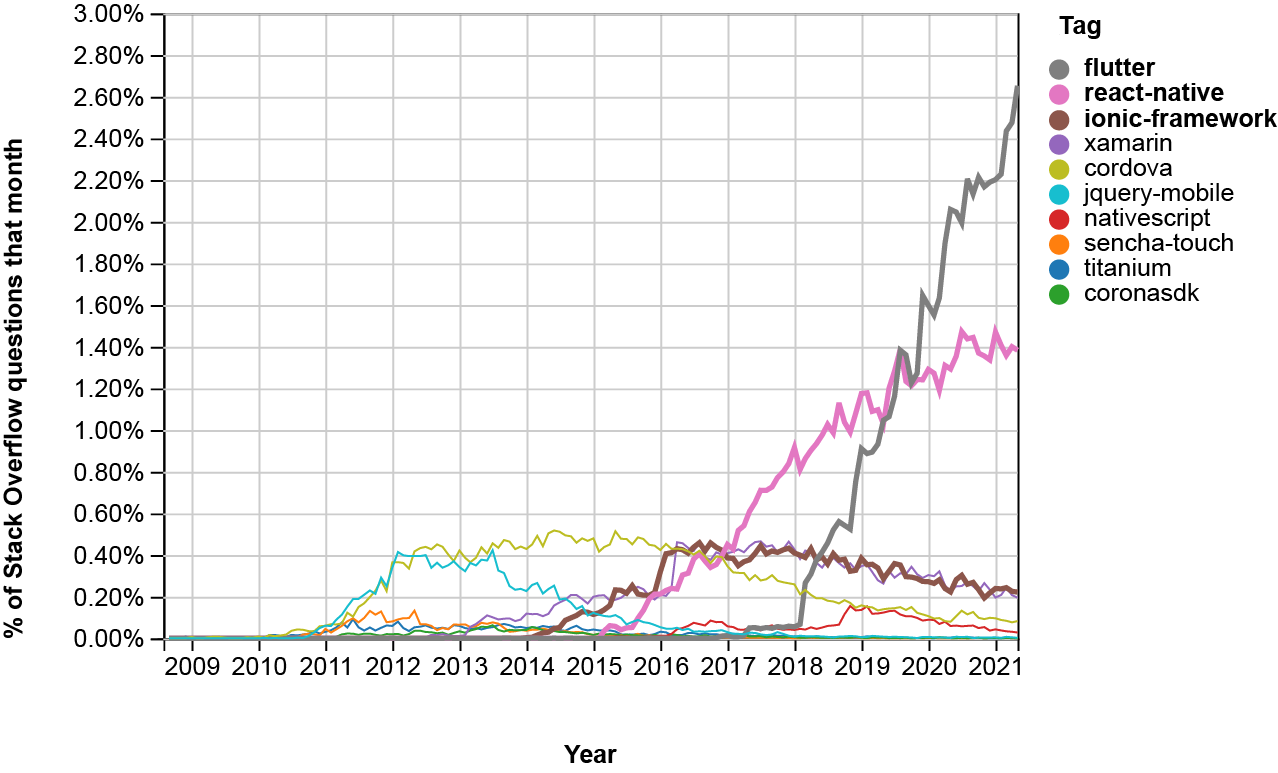
\includegraphics[scale=0.5]{framework_trends}
	\centering
	\caption{Verteilung der gestellten Fragen auf StackOverflow ausgewählter Frameworks}
\end{figure}

Auf dieser Grundlage wurden die drei populärsten Frameworks ausgewählt auf die im Folgenden näher eingegangen wird.

\newpage

\section{Das Hybride Framework Ionic}

Ionic ist ein Open Source cross-plattform Framework welches 2013 von dem Startup Drifty veröffentlicht wurde. Eine Ionic App nutzt Web-Technologien wie \ac{HTML}, \ac{CSS}, TypeScript und baut auf AngularJS und Apache Cordova auf\cite{wiki_intro}. \\

Es kann flexibel für hybride Apps und \ac{PWA}s verwendet werden. Der Fokus von Ionic liegt auf dem Frontend. Zunächst aufbauend auf dem Angular Framework stellt Ionic \ac{UI}- Komponenten für z.B. Listen, Buttons, Layouts bereit, welche den nativen Gegenstücken nachempfunden sind. Technisch bildet dabei Apache Cordova die Schnittstelle für plattformspezifische Funktionalitäten als auch die Grundlage, um plattformunabhängige Applikationen erstellen zu können. Seit Version 4 ist Ionic nicht mehr fest an AngularJS gekoppelt und es können beliebige Front-End-Frameworks wie React oder Vue benutzt werden, sowie Ionics eigene Komponenten, ohne spezifisches Front-End-Framework. Außerdem kann statt Apache Cordova Ionics eigene Laufzeitumgebung Capacitor genutzt werden, um die Anwendung auf einem Endgerät auszuführen\cite{ionic_docs}\cite{ionic_intro}.\\

	\begin{figure}[h]
		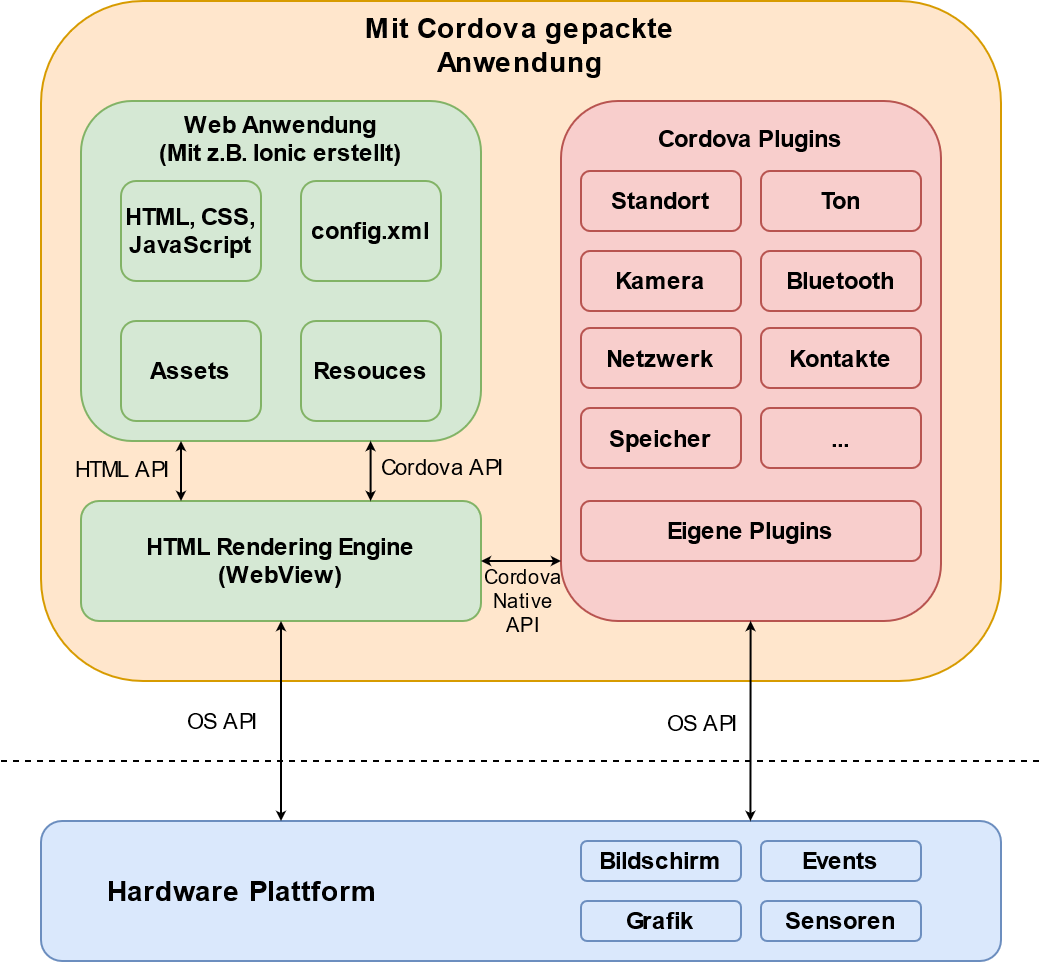
\includegraphics[scale=0.25]{cordova_ionic}
		\centering
		\caption[Übersicht einer mit Cordova gepackten App]{Übersicht einer mit Cordova gepackten App (Anlehnung an \cite{cordova_diagramm} )}
	\end{figure}

\newpage

Die Komponenten der Applikation werden mit \ac{HTML} definiert, mit \ac{SASS}, einem Superset von \ac{CSS} mit Zusatzfunktionen, gestyled und deren verhalten mit JavaScript oder optional mit TypeScript definiert. Die Sprache TypeScript wurde von dem Angular Framework übernommen und stellt ein Superset von JavaScript dar, welche einige zusätzliche Sprachfeatures als auch ein Typsystem bietet. Die mit TypeScript definierten Komponenten werden zu JavaScript tanspiliert, sodass Typfehler während des Kompilierens identifiziert werden können. Die mit Ionic gebauten Anwendungen können über die Plattform spezifischen App-Stores ausgeliefert, oder als Web-App verfügbar gemacht werden.

\begin{figure}[h]
	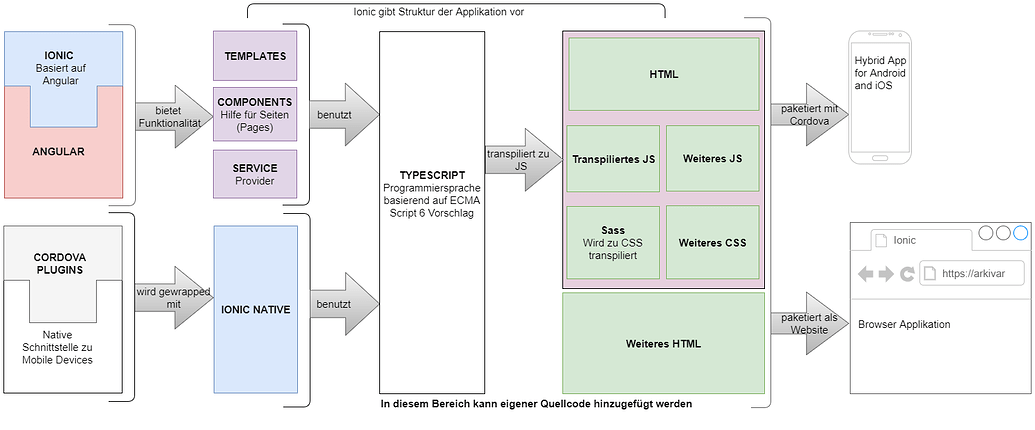
\includegraphics[scale=0.46]{ionic_flow_arkivar}
	\centering
	\caption[Übersicht der verwendeten Technologien einer Ionic App]{Übersicht der verwendeten Technologien einer Ionic App\cite{ionicForum_diagramm}}
\end{figure}

Werden bei der Entwicklung die angebotenen Komponenten genutzt, entsteht ein einheitliches Design, zudem ein umfassendes Theming viele Aspekte der Gestaltung bereits abnimmt. Jedoch kann dies auch zu einem Nachteil werden, vor allem dann, wenn Abweichungen von den Standardkomponenten gefordert sind. Ebenfalls als Nachteil ist hierbei die Performance von Ionic zu nennen, da im Gegensatz zu anderen Frameworks welche native \ac{UI}-Komponenten verwenden, diese hierbei im WebView gerendert werden\cite{altexsoft_comparison}.

\newpage
\section{React Native - Framework mit eigenständiger Laufzeitumgebung}
\label{react}
React Native wurde 2013 während eines Facebook internen Hackathon entwickelt und im Mai 2015 veröffentlicht, wobei zunächst nur iOS unterstützt wurde. Die Android-Unterstützung folgte wenige Monate später. React Native baut auf der \ac{API} des populären und ebenfalls von Facebook entwickelten JavaScript Framework React auf. Dieses wurde 2013 für Web-Anwendungen entwickelt und legt den Fokus auf die Darstellung von Komponenten abhängig von den zur Verfügung gestellten Daten des Anwenders oder der Anwendung. React Native übernimmt die Prinzipien von ReactJS, sodass jemand der mit ReactJS vertraut ist ohne Probleme auf React Native umsteigen könnte. Die gesamte Anwendung, zusammen mit den \ac{UI}-Komponenten wird mit JavaScript oder optional TypeScript, zusammen mit der eigenen Templating Syntax JSX geschrieben. React Native stellt in erster Linie abstrakte \ac{UI}-Komponenten bereit, welche anschließend auf das jeweilige Gegenstück der Zielplattform abgebildet werden. Somit kann eine Button-Komponente, wie jede andere React-Komponente, direkt in dem JavaScript Code importiert und verwendet werden. Diese hat auf der entsprechenden Plattform ein natives Gegenstück, welches gerendert wird\cite{rieger_evaluation}\cite{hansen_performance_overhead_cross_platform}\cite{droids_react_intro}.\\

React Native selbst besteht aus nativen Komponenten für die jeweilige Plattform, einer JavaScript Laufzeitumgebung, und der React Native Bridge\cite{react_intro_book}.

\begin{itemize}
	\vspace{-2mm}
	\setlength\itemsep{0mm}
	\item Die nativen Komponenten sind in der Sprache der jeweiligen Plattform geschrieben. Diese stellen die Funktionen und UI-Komponenten für den in JavaScript geschriebenen Anwendungscode bereit.
	\item Die JavaScript Laufzeitumgebung führt die eigentliche Anwendungslogik auf dem Endgerät aus. Bei iOS Geräten nutzt React Native die JavaScriptCore Laufzeitumgebung, welche vom Betriebssystem bereitgestellt wird. Diese wird ebenfalls von Safari verwendet und ist somit bereits auf dem Gerät vorhanden. Bei der Android Zielplattform hingegen, wird JavaScriptCore zusammen mit der Applikation ausgeliefert, da diese nicht vom Betriebssystem bereitgestellt werden kann. Die führt zu einer erhöhten Anwendungsgröße von React Native Anwendungen unter Android.
	\item Um die Kommunikation zwischen dem von Anwendungsentwickler geschriebenen JavaScript Code und den nativen Komponenten zu ermöglichen, wird die sogenannte React Native Bridge verwendet. Diese reagiert auf Eingaben des Benutzers, welche in dem nativen Teil der Applikation registriert werden, übersetzt diese in deren JavaScript äquivalent, damit der Anwendungscode diese verarbeiten und darauf reagieren kann. Diese Reaktion wird nun wiederum von einer JavaScript Anweisung in das native äquivalent abgebildet und dem User angezeigt.
\end{itemize}

\newpage

\begin{figure}[h]
	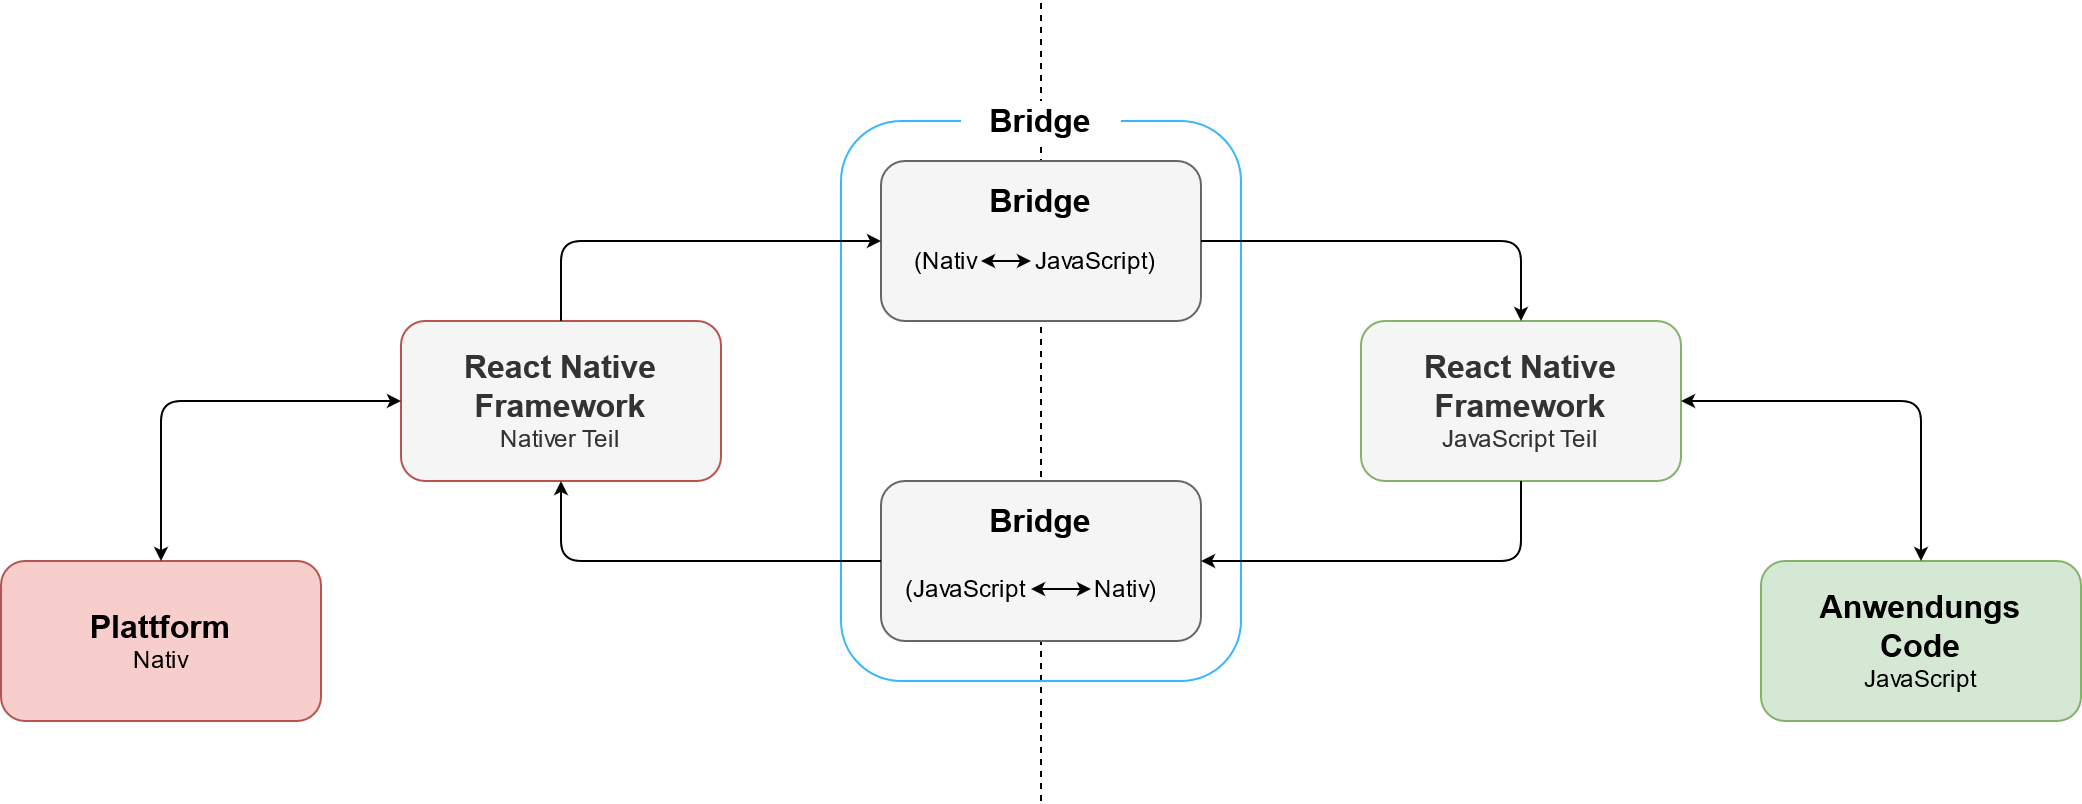
\includegraphics[scale=0.2]{react_bridge}
	\centering
	\caption[Übersicht der Kommunikation des React Frameworks]{Übersicht der Kommunikation zwischen dem Nativen- und JavaScript-Teil des React Frameworks (Anlehnung an \cite{droids_react_intro})}
\end{figure}

Da die gesamte Kommunikation des nativen und des JavaScript Teils über die React Native Bridge laufen, stellt diese einen Engpass dar, welcher zu Performanceeinbußen führt. Vor allem bei Animationen, welche z.B. von der Position des Fingers des Users abhängig sind, muss bis zu 60-mal pro Sekunde über die Bridge kommuniziert werden.

\blockcquote{talKol_react_performance}{
Here lies one of the main keys to understanding React Native performance. Each realm by itself is blazingly fast. The performance bottleneck often occurs when we move from one realm to the other. In order to architect performant React Native apps, we must keep passes over the bridge to a minimum.
}

Um dieses Problem zu beheben, arbeitet das React Native Team derzeit an einer grundlegend neuen Architektur. Diese trägt den Projektnamen Fabric\cite{react_fabric_youtube}.

\newpage
\section{Das Cross-Kompilierende Framework Flutter}

Flutter ist ein von Google entwickeltes Open Source cross-plattform \ac{SDK}, um nativ kompilierte Anwendungen für Web, Desktop und Mobilgeräte ausgehend von einer einzigen Codebasis zu entwickeln. Es wurde 2018 offiziell veröffentlicht und benutzt die ebenfalls von Google entwickelte Programmiersprache Dart\cite{flutter_dev}.\\

Dart ist eine ECMA-Standardisierte Vielzweck-Programmiersprache und wurde ursprünglich als alternative zu JavaScript entwickelt\cite{techcrunch_dart}. Dart ist optional typisiert, somit kennt Dart zwei Laufzeit-Modi: Produktion und Checked. Im Produktionsmodus wählt der Compiler selbstständig einen Typen und ignoriert Typisierungsanweisungen sowie Typfehler, um eine möglichst hohe Effizienz zu gewährleisten. Im Checked-Modus werden Typen strikt beachtet und bei Fehlern Exceptions geworfen. Die dafür notwendige Codeanalyse macht diesen Modus jedoch langsamer. Dart kann je nach Verwendungszweck auf verschiedene Arten kompiliert werden. Dazu gehören für die native Entwicklung \ac{JIT}, \ac{AOT} sowie der dart2js und dartdevc Compiler, welcher aus Dart Code JavaScript für das Web erzeugt\cite{dart_dev}.\\

\begin{figure}[h]
	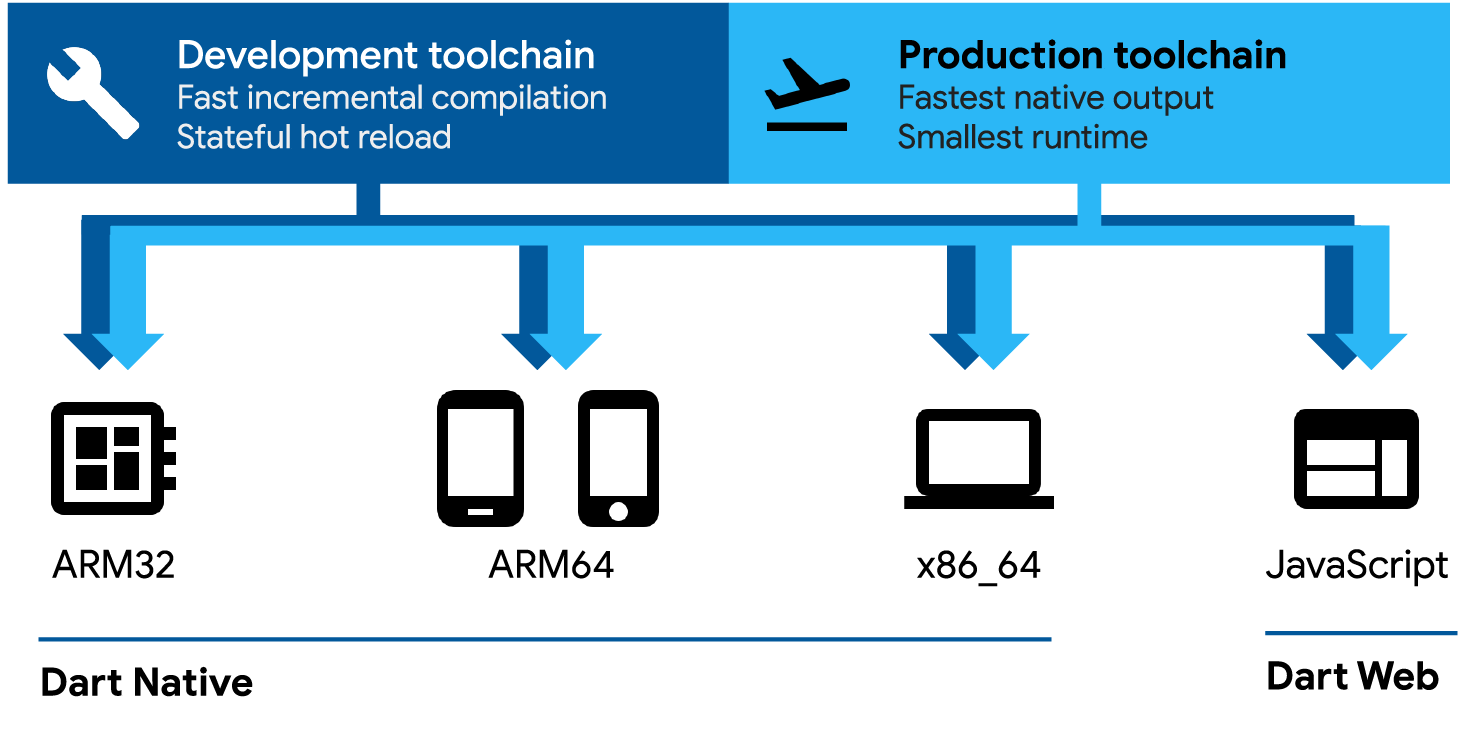
\includegraphics[scale=0.4]{dart_platforms}
	\centering
	\caption[Übersicht der Zielplattformen der Programmiersprache Dart]{Übersicht der Zielplattformen der Programmiersprache Dart \cite{dart_dev}}
\end{figure}


Diese Flexibilität macht Dart einzigartig, in der Hinsicht, dass es die einzige breit verwendete Programmiersprache ist, welche diese Möglichkeiten bietet. Bei der Entwicklung wird meist der \ac{JIT} Ansatz zusammen mit einer Dart \ac{VM} verwendet, da damit der Entwicklungsfluss gefördert wird, da Anpassungen im Quellcode direkt beobachtet werden können. Zum Ausliefern der Anwendung wird diese schließlich \ac{AOT} kompiliert. Der Vorteil von \ac{AOT} kompiliertem Code ist, dass dadurch die Startzeit der Anwendung stark verringert werden kann. Anwendungen, welche den Code zuerst kompilieren müssen, haben aufgrund der notwendigen Codeanalyse und der Kompilation selbst eine längere Startzeit. Es wurde nachgewiesen, dass bei längeren Verzögerungen, User von der Benutzung einer App oder Website absehen, falls die Ladezeit drei Sekunden übersteigt\cite{akamai_abandonment}. Ein weiterer Vorteil des \ac{AOT} Ansatzes ist, dass damit dem Problem der \glqq JavaScript Bridge\grqq\ entgegengewirkt wird. Dieses entsteht durch die Notwendigkeit der Kommunikation zwischen einer dynamischen und somit \ac{JIT} kompilierten Sprache wie JavaScript sowie dem nativen Code der Plattform.\\

Dieses Problem wird durch die \ac{AOT} Kompilation von Dart zwar nicht komplett beseitigt, da dieser ebenfalls über ein Interface mit dem nativen Code kommunizieren muss, jedoch muss kein kompletter Kontextwechsel vollzogen werden. Da Flutter die \ac{UI}-Komponenten selbst mithilfe der mitgelieferten Skia Engine rendert ist die Notwendigkeit häufiger Kommunikation ebenfalls geringer und dadurch ressourcenschonender.
Die Tatsache, dass die \ac{UI}-Komponenten (bei Flutter Widgets genannt) von der Applikation und nicht von der Plattform gerendert werden birgt einige Vorteile. Einerseits sind die UI-Komponenten erweiterbar und anpassbar, andererseits entfällt die Notwendigkeit eines virtuell \ac{DOM}s. Dieser ist bei Frameworks wie React die Grundlage, um die interne Repräsentation des Inhaltes darzustellen und wird bei Veränderungen mit dem tatsächlichen \ac{DOM} verglichen, sodass Unterschiede gebündelt angepasst werden können. Da Flutter die \ac{UI}-Komponenten selber rendert, entfällt die Notwendigkeit und der damit verbundene Aufwand, da der virtuelle \ac{DOM} gleichzeitig den reellen \ac{DOM} darstellt.
Andererseits steigt durch die Tatsache, dass Flutter die UI-Komponenten und den passenden Renderer bereitstellt die Kompatibilität der verschiedenen Betriebssystemversionen. Die Notwendigkeit auf all diesen Versionen testen zu müssen entfällt, da sich die Flutter-Entwickler darum kümmern.
Der Dart Code einer Flutter Anwendung kommuniziert mittels der sogenannten Platform Channels mit dem nativen API der Plattform. Dabei werden keine Abbildungen von Dart Code zu nativen \ac{API}-Aufrufen verwendet, sondern bidirektionale Nachrichten, welche asynchron verarbeitet werden und mithilfe von Callbacks dem Aufrufer ihr Ergebnis mitteilen. Dadurch entfällt der Engpass der zentralen Bridge.\\

\begin{figure}[h]
	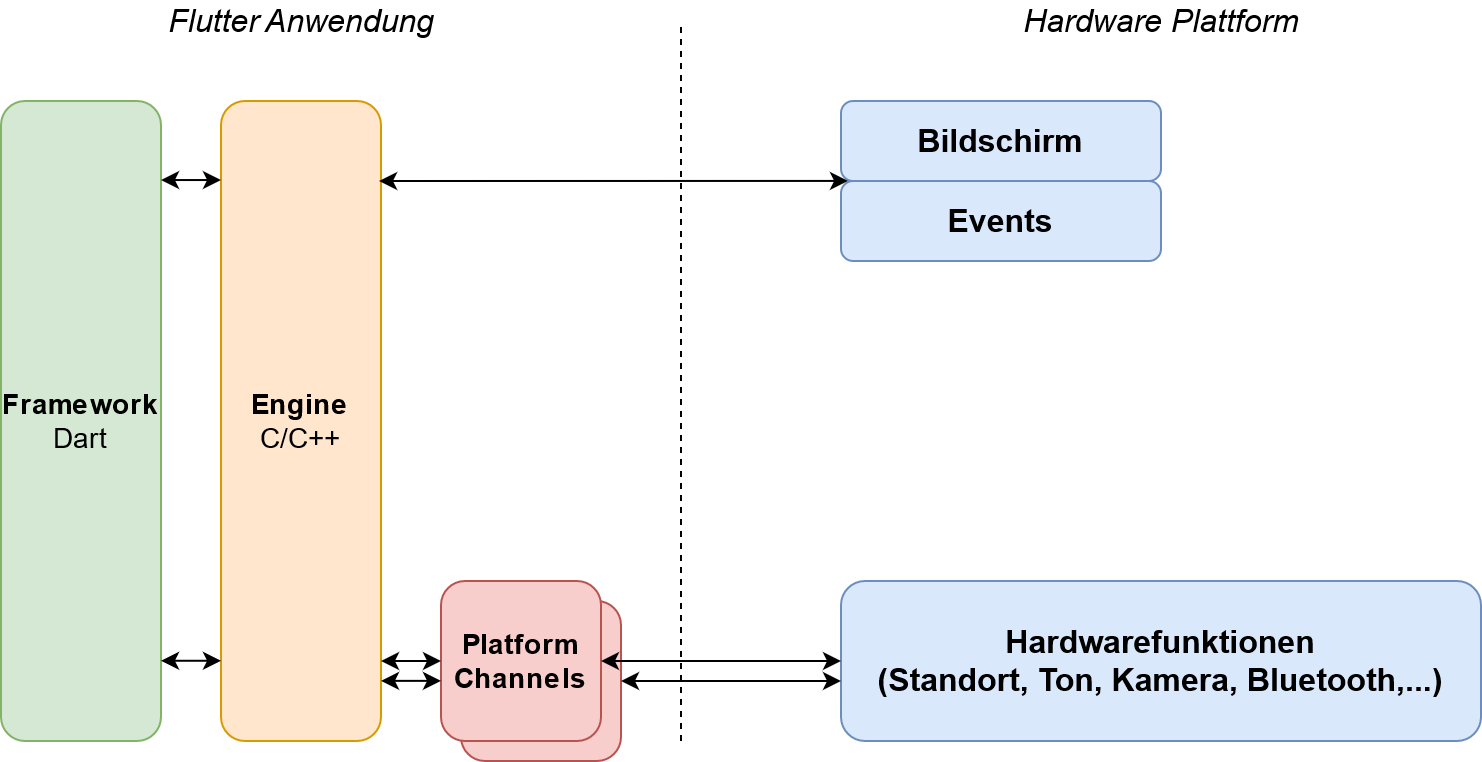
\includegraphics[scale=0.2]{flutter_architecture}
	\centering
	\caption{Vereinfachtes Schema einer Flutter Anwendung}
\end{figure}

Im Allgemeinen ähnelt das Flutter Framework einer Game Engine. Da Flutter Anwendungen aus dem Framework selbst (Dart), einer performanten Rendering Engine (C/C++) und einem plattformspezifischen Teil bestehen, welcher den Einstiegspunkt der Anwendung bildet und sich um die Kommunikation mit dem Betriebssystem kümmert.


